% % % % % % % % % % % % % % % % % % % % % % % % % % % % % % % % % % % % % % % % % % % %
%                                                                                     %
% Short Sectioned Assignment LaTeX Template Version 1.0 (5/5/12)                      %
% This template has been downloaded from: http://www.LaTeXTemplates.com               %
%                                                                                     %
% Original author:  Frits Wenneker (http://www.howtotex.com)                          %
%                                                                                     %
% Modified by: Fco Javier Sueza Rodríguez (fcosueza@disroot.org)                      %
%                                                                                     %
% Changes:                                                                            %
%	    - Custom Chapters, Sections and Subsections (titlesec package)                %
%           - Document type scrbook (oneside)                                         %
%           - Use babel-lang-spanish package and marvosym                             %
%           - Use hyperref, enumitem, tcolorbox and glossaries packages               %
%           - Use Time New Roman (mathptmx), Helvetic and Courier fonts               %
%                                                                                     %
% License: CC BY-NC-SA 3.0 (http://creativecommons.org/licenses/by-nc-sa/3.0/)        %
%                                                                                     %
% % % % % % % % % % % % % % % % % % % % % % % % % % % % % % % % % % % % % % % % % % % %

%-----------------------------------------------%
%	              Packages                  %
%-----------------------------------------------%

\documentclass[paper=a4, fontsize=11pt, oneside]{scrbook}

% ---- Text Input/Output ----- %

\usepackage[T1]{fontenc}
\usepackage[utf8]{inputenc}
\usepackage{mathptmx}
\usepackage[scaled=.92]{helvet}
\usepackage{courier}
\usepackage[indent=12pt]{parskip}

\usepackage{geometry}
\geometry{verbose,tmargin=3cm,bmargin=3cm,lmargin=2.6cm,rmargin=2.6cm}

% ---- Language ----- %

\usepackage[spanish]{babel}
\usepackage{marvosym}

% ---- Another packages ---- %

\usepackage{amsmath,amsfonts,amsthm}
\usepackage{graphics,graphicx}
\usepackage{titlesec}
\usepackage{fancyhdr}
\usepackage{tcolorbox}
\usepackage{hyperref}
\usepackage{enumitem}
\usepackage[automake]{glossaries}

%--------------------------------------------------------------------%
%                      Customizing Document                          %
%--------------------------------------------------------------------%


% ----------- Custom Chapters, Sections and Subsections -------------- %

\titleformat{\chapter}[display]
			{\bfseries\Huge}
			{Tema \ \thechapter} {0.5ex}
			{\vspace{1ex}\centering}

\titleformat{\section}[hang]
			{\bfseries\Large}
			{\thesection}{0.5em}{}

\titleformat{\subsection}[hang]
			{\bfseries\large}
			{\thesubsection}{0.5em}{}

\titleformat{\subsubsection}[hang]
			{\bfseries\large}
			{\thesubsubsection}{0.5em}{}

\hypersetup{
    colorlinks=true,
    linkcolor=black,
    urlcolor=magenta
}

% ------------------- Custom heaaders and footers ------------------- %

\pagestyle{fancyplain}

\fancyhead[]{}
\fancyfoot[L]{}
\fancyfoot[C]{}
\fancyfoot[R]{\thepage}

\renewcommand{\headrulewidth}{0pt} % Remove header underlines
\renewcommand{\footrulewidth}{0pt} % Remove footer underlines

\setlength{\headheight}{13.6pt} % Customize the height of the header

% --------- Numbering equations, figures and tables ----------------- %

\numberwithin{equation}{section} % Number equations within sections
\numberwithin{figure}{section} % Number figures within sections
\numberwithin{table}{section} % Number tables within sections

% ------------------------ New Commands ----------------------------- %

\newcommand{\horrule}[1]{\rule{\linewidth}{#1}} % Create horizontal rule command


%----------------------------------------------------------------------------------------
%	TÍTULO Y DATOS DEL ALUMNO
%----------------------------------------------------------------------------------------

\title{
\normalfont \normalsize
\textsc{{\bfseries Curso 2023-2024} \\ Ciclo Superior de Desarrollo de Aplicaciones Web \\ IES Aguadulce} \\ [25pt]
\horrule{0.5pt} \\[0.4cm]
\huge Empresa e Iniciativa Emprendedora \\
\horrule{0.5pt} \\[0.4cm]
}

\author{Francisco Javier Sueza Rodríguez}
\date{\normalsize\today}

%----------------------------------------------------------------------------------------
%                                     DOCUMENTO
%----------------------------------------------------------------------------------------
\makeglossaries
\loadglsentries{glossary.tex}

\begin{document}

\maketitle

\newpage

\tableofcontents

\listoffigures

%\listoftables

\newpage

\chapter{La Empresa y su Clasificación}
En este primer tema, vamos en que consiste una empresa, dando su definición y explicando los diferentes elementos que la componen, tanto humanos como materiales, así como de su organización. También hablaremos sobre la función y finalidad que tiene una empresa, hablaremos de la ética empresarial y daremos una clasificación de la empresa según diferentes características.

\section{Empresa e Iniciativa Emprendedora}
En este módulo pretendemos \textbf{conocer más sobre la empresa}. A diferencia de la asignatura de \textbf{Formación y Orientación Laboral}, donde se adopta el punto de vista del trabajador, nosotros adoptaremos el punto de vista del empresario o empresaria, porque tu también puede llegar a serlo, y porque, aunque trabajes por cuenta ajena, también necesita saber como colaborar para que tu empresa pueda mejorar.

El concepto de empresa puede ser definido desde ópticas muy diferentes: llamamos empresa al lugar de trabajo, a una acción o tarea que entrañe dificultades y cuya ejecución requiere decisión y esfuerzo, a la unidad organizada que desarrolla una actividad económica, etc. Partiendo de esta última perspectiva, vamos a definir la empresa.

Una \textbf{empresa} es un conjunto de \textbf{elementos humanos y materiales organizados} dedicado a la \textbf{producción de bienes} y/o la prestación de \textbf{servicios} dirigidos a satisfacer necesidades humanas, con ánimo de obtener un \textbf{beneficio}.

\section{Elementos de una Empresa}
Podemos establecer, de una forma muy simplificada, que los elementos de una empresa son los que podemos ver en la siguiente figura.

\begin{figure}[H]
    \centering
    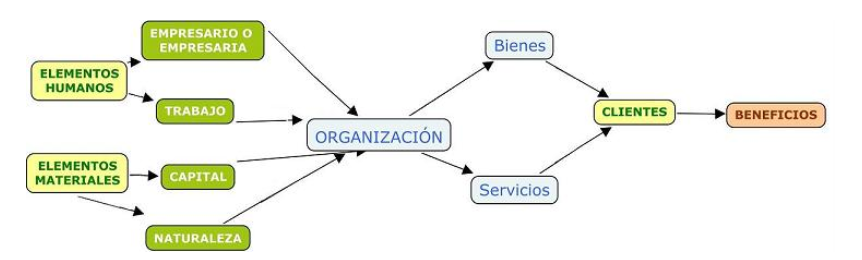
\includegraphics[scale=0.50]{elementos-empresa.png}
    \caption{Elementos de una empresa}
\end{figure}

En los siguiente puntos, vamos a analizaremos algunos de estos elementos.

\subsection{Los Elementos Humanos}
En primer lugar, vamos a ver cuales son los elementos humanos que componen una empresa, pudiendo diferenciar principalmente entre los siguientes dos elementos:

\begin{itemize}
    \item \textbf{Empresaria o Empresario}: es la persona o grupo de éstas que aporta \textbf{el capital} para el desarrollo de la actividad empresarial y asume \textbf{los riesgos} que de ella se deriven con la intención de obtener un beneficio económico.

    \item \textbf{Trabajadores y Trabajadoras}: tradicionalmente llamados recursos humanos, a nosotros nos gusta más llamarlo equipo de trabajo. Se trata de las personas que dedican su tiempo y esfuerzo a las actividades productivas a cambio de una remuneración, de una \textbf{salario}. Comprende cualquier tipo de \textbf{actividad humana}, ya sea física o intelectual y muy diferentes niveles de cualificación: trabajadores no cualificados, técnicos, mandos intermedios, directivos, etc.
\end{itemize}

\subsection{Los Elementos Materiales}
Los principales elementos materiales de una empresa son los recursos naturales y el capital, que describimos a continuación.

\begin{itemize}
    \item \textbf{Recursos Naturales}: son recursos naturales elementos como el agua, energía, arboles, animales, viento, etc...

    \item \textbf{Capital}: se puede considerar capital  al dinero, acciones, patentes, marcas, edificios, instalaciones, maquinarias, productos semielaborados y los demás medios materiales que intervienen en el proceso de producción. Pueden ser duraderos o no duraderos en el tiempo.
\end{itemize}

\subsection{La Organización}
Para que una empresa funcione debe estar organizada. La \textbf{organización} consiste en la coordinación de los elementos humanos y materiales de que se disponen, a fin de obtener mejor rendimiento  de los mismos.

Este \textbf{rendimiento óptimo} de los recursos disponibles procura una cantidad  y calidad deseadas, de un producto o servicio, en un tiempo determinado con un mínimo de coste, de tal forma que satisfaga las necesidades del consumidor. Si la empresa esta bien organizada, decimos que es \textbf{productiva}.

Para entender lo que es el \textbf{rendimiento óptimo} vamos a ver el siguiente ejemplo:

Un restaurante va cada vez mejor y tiene muchos clientes fijos que van a comer allí todos los días. Se ha hecho un cálculo atendiendo al método y tiempos de trabajo de la empresa y se ha determinado que se puede atender al día satisfactoriamente a 40 clientes, ¿que ocurriría si intentarán atender a 50 personas o a todas las que acudan al restaurante? ¿Cómo se sentirían los trabajadores? ¿Y los clientes? ¿Es más conveniente decirles que vuelvan otro día? A la larga, intentar maximizar los rendimientos de la empresa puede tener consecuencias negativas: empeora el clima laboral, menor calidad del servicio, problemas de espacio, incumplimiento de tiempos, clientes insatisfechos y cansados de esperar, etc...

\section{Funciones de la Empresa}
Para cumplir con sus objetivos, las empresas desarrollan un serie de \textbf{actividades} diferentes que se agrupan por divisiones, áreas, departamentos,... las denominaremos, \textbf{funciones de la empresa}.

Podemos clasificar las funciones de una empresa en:

\begin{itemize}
    \item \textbf{Función comercial}: son las actividades relacionadas con la compraventa, como investigar el mercado, hacer acopio de los materiales necesarios, obtención del producto, ponerle precio, etc...
    \item \textbf{Función de producción, de operaciones o técnica}: son las actividades relativas al diseño del producto, el proceso de producción y transformación de las materias primas, gestión del almacén, etc..
    \item \textbf{Función financiera y contable}: se encarga de la obtención del capital, control de los ingresos y gatos, documentación, etc...
    \item \textbf{Función social}: tiene que ver con el equipo humano que compone la empresa, determinar que tipo de personas deben ser, los tipos de contratos que se van a realizar, etc..
    \item \textbf{Función directiva}: es la función encargada de coordinar todas las funciones anteriores, planificando y organizando todas las funciones para que la empresa pueda llegar a sus objetivos.
\end{itemize}

Para que todas estas funciones trabajen adecuadamente hay que tener en cuenta lo siguiente:

\begin{itemize}
    \item \textbf{Dependencia}: la efectividad de una empresa no depende de un área funcional específica, sino de la coordinación de todas ellas.

    \item \textbf{Graduación de la importancia}: las funciones no revisten la misma importancia en todas las empresas. A veces algunas dominan sobre el resto, incluso puede suceder que haya alguna que carezca de relevancia. Por ejemplo, en una tienda de ropa, la función más relevante es la comercial, mientras que realmente no hay una función de producción.
\end{itemize}

La \textbf{importancia de una función} va a depender de la actividad que desarrolle la empresa, el tamaño, el número de personas implicadas, etc.

Por ejemplo, en una empresa individual todas las funciones son realizadas por al misma persona, mientras que en una multinacional, con cientos de personas trabajando, las funciones se multiplican y aparecen algunas nuevas como la Investigación, Desarrollo e Innovación (I+D+I), control de calidad, seguridad, etc.

Como veremos en temas sucesivos, las funciones de la empresa se corresponden con los apartados del \textbf{plan de negocio}, pero no adelantemos acontecimientos...

\subsection{Finalidad de una Empresa: La Satisfacción de Necesidades}
Tradicionalmente se considera que la finalidad de una empresa es la obtención de beneficios, pero el beneficio no debe ser la finalidad principal del comportamiento o las decisiones de la empresa actual, sino, la razón de su existencia.

Los \textbf{beneficios son el resultado} indispensable sin el cual los negocios no pueden sobrevivir, pero una empres que considere los beneficios como su meta principal puede ser que no llegue a conseguir sus objetivos. Vamos a intentar explicarlo mejor, la \textbf{finalidad objetiva} que debe tener en cuenta una empresa moderna es la \textbf{creación de clientes}, clientes satisfechos y fieles a los productos o servicios objeto de la actividad de la empresa. La \textbf{satisfacción} de las \textbf{necesidades de los consumidores} es la base de supervivencia de la empresa y de su crecimiento futuro.

Pero los clientes y consumidores somos cada vez más exigentes y el mundo empresarial es muy competitivo. Las empresas deben conocer estas exigencias y adaptarse a los cambios, conocer su entorno, comportarse de forma ética y asumir su responsabilidad social. Es lo que vamos a ver en los siguiente apartados.

\subsection{La Cultura de Empresa y la Imagen Corporativa}
La \textbf{empresa es un sistema}, una entidad formada por una serie de elementos, con unas determinadas funciones, que se relacionan con el exterior. Pero, ¿ que b\textbf{valores y principios} sustentan las elecciones de la empresa? ¿Cómo quiere ser?

Toda empresa tiene unos \textbf{pilares básicos} a la hora de \textbf{dirigir sus actuaciones}, un conjunto de creencias, valores, principios... que rigen su funcionamiento, que son asumidos y compartidos por las personas y los grupos que la integran y que se manifiestan en la forma en la que interaccionan con otros y ellos con el entorno, es la \textbf{cultura empresarial}.

La cultura de una organización la hace \textbf{diferente} de otros y condiciona los \textbf{objetivos} que se fijan y las \textbf{estrategias} que se siguen para lograrlos. Para que la cultura de la empresa sea aceptada y asumida por el equipo humano que la integra es necesario que las personas que dirigen la organización ejerzan un \textbf{liderazgo} eficaz que garantice la interpretación correcta de los elementos culturales.

Algunas empresas orientan su cultura \textbf{al poder}, otras se preocupan de la \textbf{función}, otras se orientan a la \textbf{consecución de objetivos} y resultados fomentando, por ejemplo, la planificación y el trabajo en equipo.

En los últimos tiempos se esta incrementando el número de empresas que centran su atención en \textbf{las personas}, en el \textbf{equipo humano}, tratando de satisfaces sus necesidades sociales y potenciando su desarrollo personal y profesional. Su estructura, con \textbf{pocos niveles de autoridad}, fomenta la participación y el consenso de decisiones. El bienestar de los empleados, la realización laboral y la conciliación de la vida laboral y personal podrían ser algunos de sus valores.

La \textbf{imagen corporativa} de una empresa es la imagen que la empresa proyecta al exterior, lo que la gente piensa y siente acerca de lo que la empresa es y como actúa. El logotipo, la decoración, los uniformes de la empresa, los colores distintivos, el eslogan, la música... incluso el olor, son símbolos que trasmiten una imagen, una personalidad de la empresa y que influyen en su éxito o fracaso. Es importante, que la imagen que se perciba de la empresa este acorde con la imagen que ésta quiere transmitir.

\subsection{La Ética Empresarial}
\textbf{La ética} es la parte de la Filosofía que estudia la moral y determina que es lo bueno (o lo malo), lo correcto (o lo incorrecto), lo permitido (o no permitido) y como se debe actuar. La empresa actúa y sus actuaciones tiene unas repercusiones positivas o negativas sobre las personas que la integran y su entorno.Estos principio se recogen en un \textbf{código de conducta} que se convierte en la expresión escrita de la cultura de la empresa.

El \textbf{comportamiento no ético} en la empresa tiene muchas consecuencias negativas, entre ellas:

\begin{itemize}
    \item Desprestigio y mala imagen.
    \item Pérdida de clientes.
    \item Trabajadores descontentos, desmotivados, improductivos o que dejan la empresa.
    \item Proveedores que no quieren establecer relaciones comerciales.
    \item Bancos que no aprueban créditos.
    \item Perdida de relaciones con la Administración, perdida de posibles subvenciones o ayudas.
    \item Sanciones jurídicas, cuando además los actos no éticos incumplen las normas jurídicas.
\end{itemize}

Como vemos, las consecuencias de llevar a cabo acciones poco éticas pueden ser muchas y muy perjudiciales para una empresa.

\subsection{La Responsabilidad Social de las Empresas}


% Apéndice
\appendix

% Change appendix display options
\titleformat{\chapter}{\bfseries\Huge}{\thechapter.}{1ex}{}



% Bibliography

\addcontentsline{toc}{chapter}{Bibliografía}
\bibliography{citas}
\bibliographystyle{unsrt}

\end{document}